%\documentclass[eng, draft, openany]{mgr} %Draft
%\documentclass[eng, openany]{mgr} %Draft with img

\documentclass[eng, printmode, final]{mgr} %Print

\usepackage{polski}
\usepackage[utf8x]{inputenc}

%pakiety do grafiki
\usepackage{graphicx}
%\usepackage{subfigure}
\usepackage[caption = false]{subfig}
%\usepackage{subcaption}
\usepackage{psfrag}

%pakiety dodające dużo dodatkowych poleceń matematycznych
\usepackage{amsmath}
\usepackage{amsfonts}

%pakiety wspomagające i poprawiające składanie tabel
\usepackage{supertabular}
\usepackage{array}
\usepackage{tabularx}
\usepackage{hhline}

%pakiet wypisujący na marginesie etykiety równań i rysunków zdefiniowanych przez \label{}, chcąc wygenerować finalną wersję dokumentu wystarczy usunąć poniższą linię
\usepackage{showlabels}

\usepackage{pythonhighlight}

\usepackage{tikz}
\usetikzlibrary{trees}

%definicje własnych poleceń
\newcommand{\R}{I\!\!R} %symbol liczb rzeczywistych, działa tylko w trybie matematycznym
\newtheorem{theorem}{Twierdzenie}[section] %nowe otoczenie do składania twierdzeń

%dane do złożenia strony tytułowej
\title{Zastosowanie algorytmów fotogrametrii dla estymacji położenia obserwatora w przestrzeni trójwymiarowej}
\engtitle{A photogrammetric approach for observer's position estimation in 3D}
\author{Lev Sergeyev}
\supervisor{Dr hab. inż. Przemysław Śliwiński}
%\guardian{? Prof. dr hab. inż. Czesław Smutnicki, prof. PWr}

\date{2020} %standardowo u dołu strony tytułowej umieszczany jest bieżący rok, to polecenie pozwala wstawić dowolny rok

\field{Automatyka i Robotyka (AIR)}
\specialisation{Systemy informatyczne w automatyce (ASI)}


%%%%%%%%%%%%%%%%%%%%%%%%%%
%% DOCUMENT:            %%
%%%%%%%%%%%%%%%%%%%%%%%%%%

\begin{document}
%\bibliographystyle{plabbrv} %tylko gdy używamy BibTeXa, ustawia polski styl bibliografii

\maketitle

\tableofcontents
\listoffigures
% \listoftables

\relax


\chapter{Wstęp}
Praca jest podzielona na pięć rozdziałów. W tym rozdziale są rozpatrzone problem który spróbowano rozwiązać i pytania na które spróbowano dać odpowiedź. Trzy następne rozdziały opisują przebieg pracy. Ostatni rozdział jest poświęcony analizie przerobionej pracy.

\section{Problem lokalizacji}

W wielu sferach życia, jak i w procesach technologicznych występuje potrzeba określenia położenia w przestrzeni --- lokalizacji. To może dtyczyć jak wyznaczania położenia obserwatora tak i lokalizacja obiektu.

W tej pracy proponowanym rozwiązaniem problemu lokalizacji jest stosowanie \textbf{pozycjonowania fotogrametrycznego}. Taki rodzaj lokalizacji polega na szacowaniu pozycji obserwatora(obiektywu kamery) względem sceny na podstawie dwóch lub więcej zdjęć. Pozycjonowanie na podstawie zdjęć przewiduje także obecności ruchomej kamery względem sceny.

Zaproponowane rozwiązanie umożliwiło by lokalizację w takich miejscach i przypadkach, gdzie korzystanie z takich narzędzi i rozwiązań jak na przykład \textbf{nawigacja satelitarna}, lokalizacja za pomocą sieci \textbf{stacji BTS}, \textbf{systemy radiolokacji}, \textbf{systemy sonarowe} staje się niemożliwym lub małoskutecznym.

Podejście fotogrametryczne w pozycjonowaniu mogłoby pozwolić na dopełnienie już istniejących systemach lokalizacji w celach zwiększenia dokładności i niezawodności systemu.

Takie podejście też mogłoby pozwolić rozbudowę funkcjonalności lokalizacji systemów już posiadających kamerę. Zaletą takiego rozwiązania może być niski koszt rozbudowy, brak konieczności przerobienia układów systemu, elastyczność konfiguracji.

Przykłądem takich systemów może być dron, robot lub pojazd autonomiczny.

Wadą zastosowania pozycjonowania fotogrametrycznego mogą być małe możliwości zasobów obliczeniowych lub

\textbf{Podejście fotogrametryczne} może być zastosowane jak dla \textbf{lokalizacji absolutnej} (kiedy znany jest układ odniesienia i skale odległośći) tak i  \textbf{lokalizacji względnej}. W rozprawie, jednak, rozpatrzono tylko lokalizację względną. Oznacza to, że rzeczywista pozycja obserwatora, pozycja sceny, skala odległości pozostają nieznane. W rozdziale 5 będzie zaproponowany sposób przejścia od lokacji względnej do lokacji absolutnej.

\pagebreak

\section{Cel pracy}

Jednym z zadań pracy była implementacja śródowiska, które umożliwia: wyznaczenie pozycji obserwatora względem sceny na podstawie zdjęć, odtworzenie sceny fotogrametrycznej i przedstawienie wyników przetwarzania w czytelny sposób.
Dodadtkowo śródowisko fotogrametryczne powinno umożliwić porównywanie wyników przetwarzania.

Kolejnym zadaniem było użyć gotowe śródowisko użyć przedwarzania róźnych zestawów danych przy róźnych parametrach i przeprowadzić analizę uzyskanych wyników.

Także w tej rozprawie podjęta próba dania odpowiedzi na takie pytania:
\begin{itemize}
   \item Czy można i w jaki sposób wyznaczyć względną pozycję kamery na podstawie zbioru zdjęć,
   \item Jaki jest algorytm zastosowanego pozycjonowania,
   \item Jakich rozwiązań można użyć dla estymacji położenia,
   \item Jakie zasoby są w stanie przeprowadzić obliczenia dla lokalizacji,
   \item Ile czasu zajmują obliczenia dla otzymania zadowalającego wyniku,
   \item Jak zależą czas i wynik lokalizacji od danych wejściowyc i parametrów fotogrammetryzacji
\end{itemize}

\graphicspath{ {./img/2_Theory/} }


\chapter{Fotogrametria. Wprowadzenie teoretyczne}

Fotogrametria - dziedzina nauki, sztuki i technologia mająca na celu wyznaczanie informacji i odtworzanie kształtów jednego lub więcej obiektu fizycznego na podstawie zdjęć obiektu.
Fotogrametria można podizelić na dwa rodzaje: płaską i przestrzenną. Fotogrametria płaska wymaga co najmniej jednego zdjęcia i jej wynikiem jest charakterystyka obiektu w płaszczyźnie. Fotogrametria przestrzenna wymaga dwóch lub więcej zdjęć, jest używana do odtwarzania obiektów w przestrzeni trójwymiarowej.

W tej pracy stosowana jest wyłącznie fotogrametria przestrzenna.

Pozwala wyznaczyć takie charakterystyki jak:
\begin{itemize}
   \item krszałt
   \item rozmiar
   \item położenie wzajemne w przestrzeni
   \item color i teksturę
\end{itemize}

Dodatkowo technologia fotogrametrii pozwala na wyznaczenie położenia kamery (obserwatora) w chwili robienia zdjęcia fotogrametrycznego.
Położenie kamery w przestrzeni trójwymiarowej jest wyznaczane na podstawie bazy sceny i wybranego zdjęcia zawierającego całość lub część sceny.

\textbf{Cecha}, punkt kluczowy --- element charakterystyczny obiektu wyróżniający się na tyle, aby można było zidentyfikować ten sam element na zdjęciu z innego ujęcia.

Pojęcie \textbf{sceny fotogrametrycznej}, często wykorzystywane w tym dokumencie, oznacza zbiór statycznych obiektów fizycznych powiązane zdjęcia których używane są do odtwarzania kształtów tego zbioru w przestrzeni trójwymiarowej. Wymaganie dla zbioru zdjęć sceny sceny jest takie, aby zdjęcia zawierały róźne ujęcia scena, przy czym posiadały jeden lub więcej elementów wspólnych i przy takich samych warunkach: oświetlenie, stan sceny, ustawienia kamery i obiektywu, taki sam aparat fotograficzny.

Odtwarzanie kształtów oznacza umieszczenie punktów charakterystycznych obiektów w przestrzeni 3D w taki sposób, aby położenie cech względem siebie odpowiadało położeniu w rezeczywistości. Odbywa się na podstawie wykrycia cech charakterystycznych, w tym ich skali, obrotu i położeniu na zdjęciu, a następnie szacowaniu położenia wspólnych cech jednej lub więcej pary zdjęć na podstawie informacji o skali, obrotu i położeniu cechy na zdjęciu.

Proponowane podejście lokalizacji kamery(obserwatora) w chwili zrobienia zdjęcia opiera się o wyznaczeniu pozycji względem cech charakterystycznych obiektu sceny.

Zaproponowany proces fotogrametryczny dla wyznaczania cech sceny i budowy sceny w przestrzeni 3D wraz z lokalizacją kamer odzwierciedla podejście wykorzystane w platformie AliceVision (opisana jest w rozdziale 3.1) dla rozwiązania analogicznego problemu. Proces ten można rozbić na poszczególne etapy, każdy etap jest opisany w rozdziałach 2.1-2.5.

\section{Wyznaczanie punktów kluczowych. Transformata SIFT}
Obraz z zestawu zdjęć fotogrametrycznych posiada cechy kluczowe które mogą być na tyle charakterystyczne, że można z wysokim prawdopodobieństwem je znaleźć w bazie cech innego zdjęcia zawierającego ten sam obiekt.

Jednym ze sposobów wyznaczania i zapisu takich elementów jest stosowanie opatentowanych algorytmów i deskryptorów \textbf{SIFT} (Scale Invariant Feature Transform - skalo-niezmienna transformata cech, Skaloniezmiennicze przekształcenie cech). Ta transformata jest powszechnie stosowana w przetwarzaniu i rozpoznawaniu obrazów do wykrywania punktów charakterystycznych.

Zastosowanie takiej transformaty na przeciętnym zdjęciu o rozmiarze 500x500 pikseli może wykryć około 2000 cech charakterystycznych, oczywiście liczba wykrytyvh elementów zależy od jak od zawartości i jakości zdjęcia, tak i od parametrów stosowanej transformaty.

Aby zminimalizować zapotrzebowanie zasobów na wyznaczanie elementów kluczowych obraz jest poddawany szeregu zabiegów optymalizacji i filtracji. Proces wyznaczania cech można przedstawić w taki szereg kroków:
\begin{enumerate}
   \item Obliczenie przestrzeni skal Gaussa
   \item Obliczenie DoG (Róźnicy filtrów Gaussa)
   \item Wyznaczenie punktów pretendujących
   \item Lokalizacja punktów kluczowych z subpikselową dokładnością
   \item Filtracja punktów niestabilnych pod względem szumu
   \item Filtracja punktów niestabilnych co leżą na krawędziach
   \item Przydział obrotu(orientacji) dla punktu kluczowego
   \item Utworzenie deskryptora punktu kluczowego
\end{enumerate}

\subsection{Filtr Gaussa}

   Także nazywany rozmyciem Gaussa --- filtr splotowy, który można zapisać w sposób konwolucji ciagłej:
   \begin{equation} \label{eq:gauss_c}
      \mathbf{F}_{g}(\mathbf{u}(\mathbf{x}))
      = (\mathbf{G}_{\sigma} * \mathbf{u}) (\mathbf{x})
      = \int \mathbf{G}_{\sigma}(\mathbf{x}') \mathbf{u}(\mathbf{x}-\mathbf{x}') d\mathbf{x}'
   \end{equation}
   gdzie $ \mathbf{u}(\mathbf{x}) , \smallskip \mathbf{x} = (x, y) \in \mathbb{R}^2 $ obraz wejściowy,
   a $ \mathbf{G}_{\sigma}(\mathbf{x}) = \frac{1}{2 \Pi \sigma^2} e^{-\frac{ | \mathbf{x} |^2}{2\sigma^2} },
   \smallskip \sigma \in \mathbb{R}^+ $ funkcja jądra konwolucji.

   W danym przypadku mamy doczynienie z obrazami rastrowymi, więc stosowany jest splot dyskretny. Konwolucja dyskretna takiego filtru z parametrem $\sigma$ dla obrazu $\mathbf{u}$ o rozmiarze $ M \times N $ ma postać:
   \begin{equation} \label{eq:gauss_d}
      \begin{split}
         \mathbf{F}_{g}(\mathbf{u}(k,l) )
         = (\mathbf{G}_{\sigma} * \mathbf{u}) (k,l) =
         \sum_{k' = -\lceil 4\sigma \rceil}^{\lceil 4\sigma \rceil} \mathbf{g}_{\sigma} (k')
         \sum_{l' = -\lceil 4\sigma \rceil}^{\lceil 4\sigma \rceil} \mathbf{g}_{\sigma} (l') \mathbf{\bar{u}} (k - k', l - l'),
         \\
         \mathbf{g}_{\sigma}(k) = Ke^{- \frac{k^2}{2 \sigma^2}}, \:
         -\lceil 4\sigma \rceil \leq k \leq \lceil 4\sigma \rceil, \:
         k \in \mathbb{Z}
      \end{split}
   \end{equation}
   gdzie $\lceil a \rceil$ --- funkcja zaokrąglająca w górę, $K$ jest takie, że $\sum \mathbf{g}_{\sigma} (k) = 1 $
   \begin{equation}
      \begin{split}
         \mathbf{\bar{u}}(k, l) =  \mathbf{\bar{u}} (s_M(k), s_N(l)),
         \\
         s_M(k) = \mathrm{min}(\mathrm{mod}(k, 2M), 2M - 1 - \mathrm{mod}(k, 2M)),
      \end{split}
   \end{equation}
   gdzie $ \mathrm{mod(a,b)} $ --- reszta z dzielenia $a$ przez $b$.

   \begin{figure}[h]
      \centering
      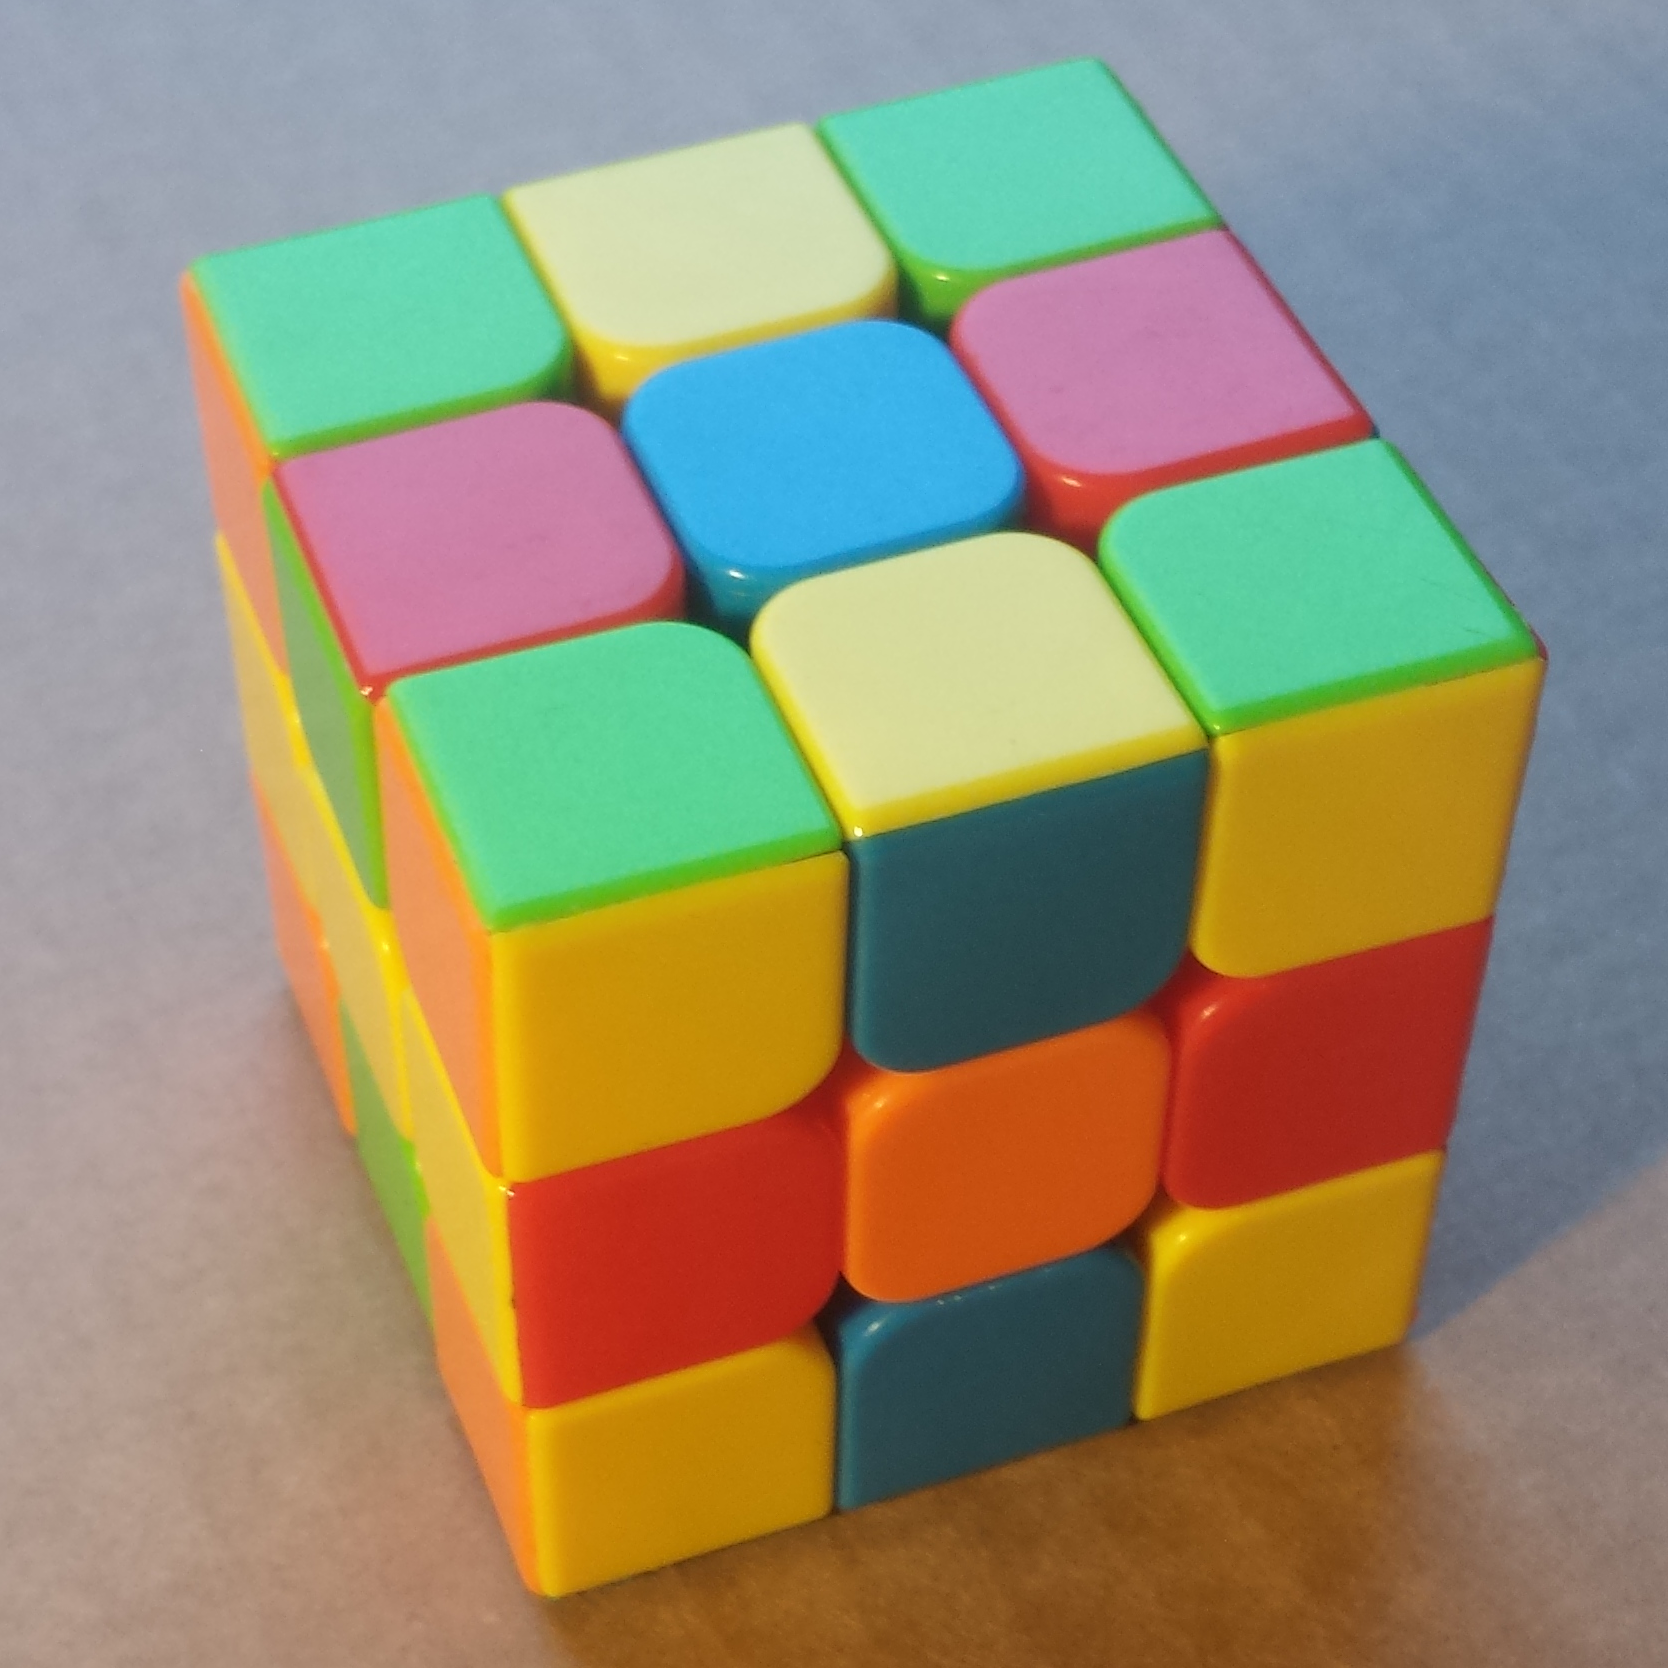
\includegraphics[width=5cm]{origin.png}
      \Large{$ \xrightarrow{\mathbf{F}_{g}} $}
      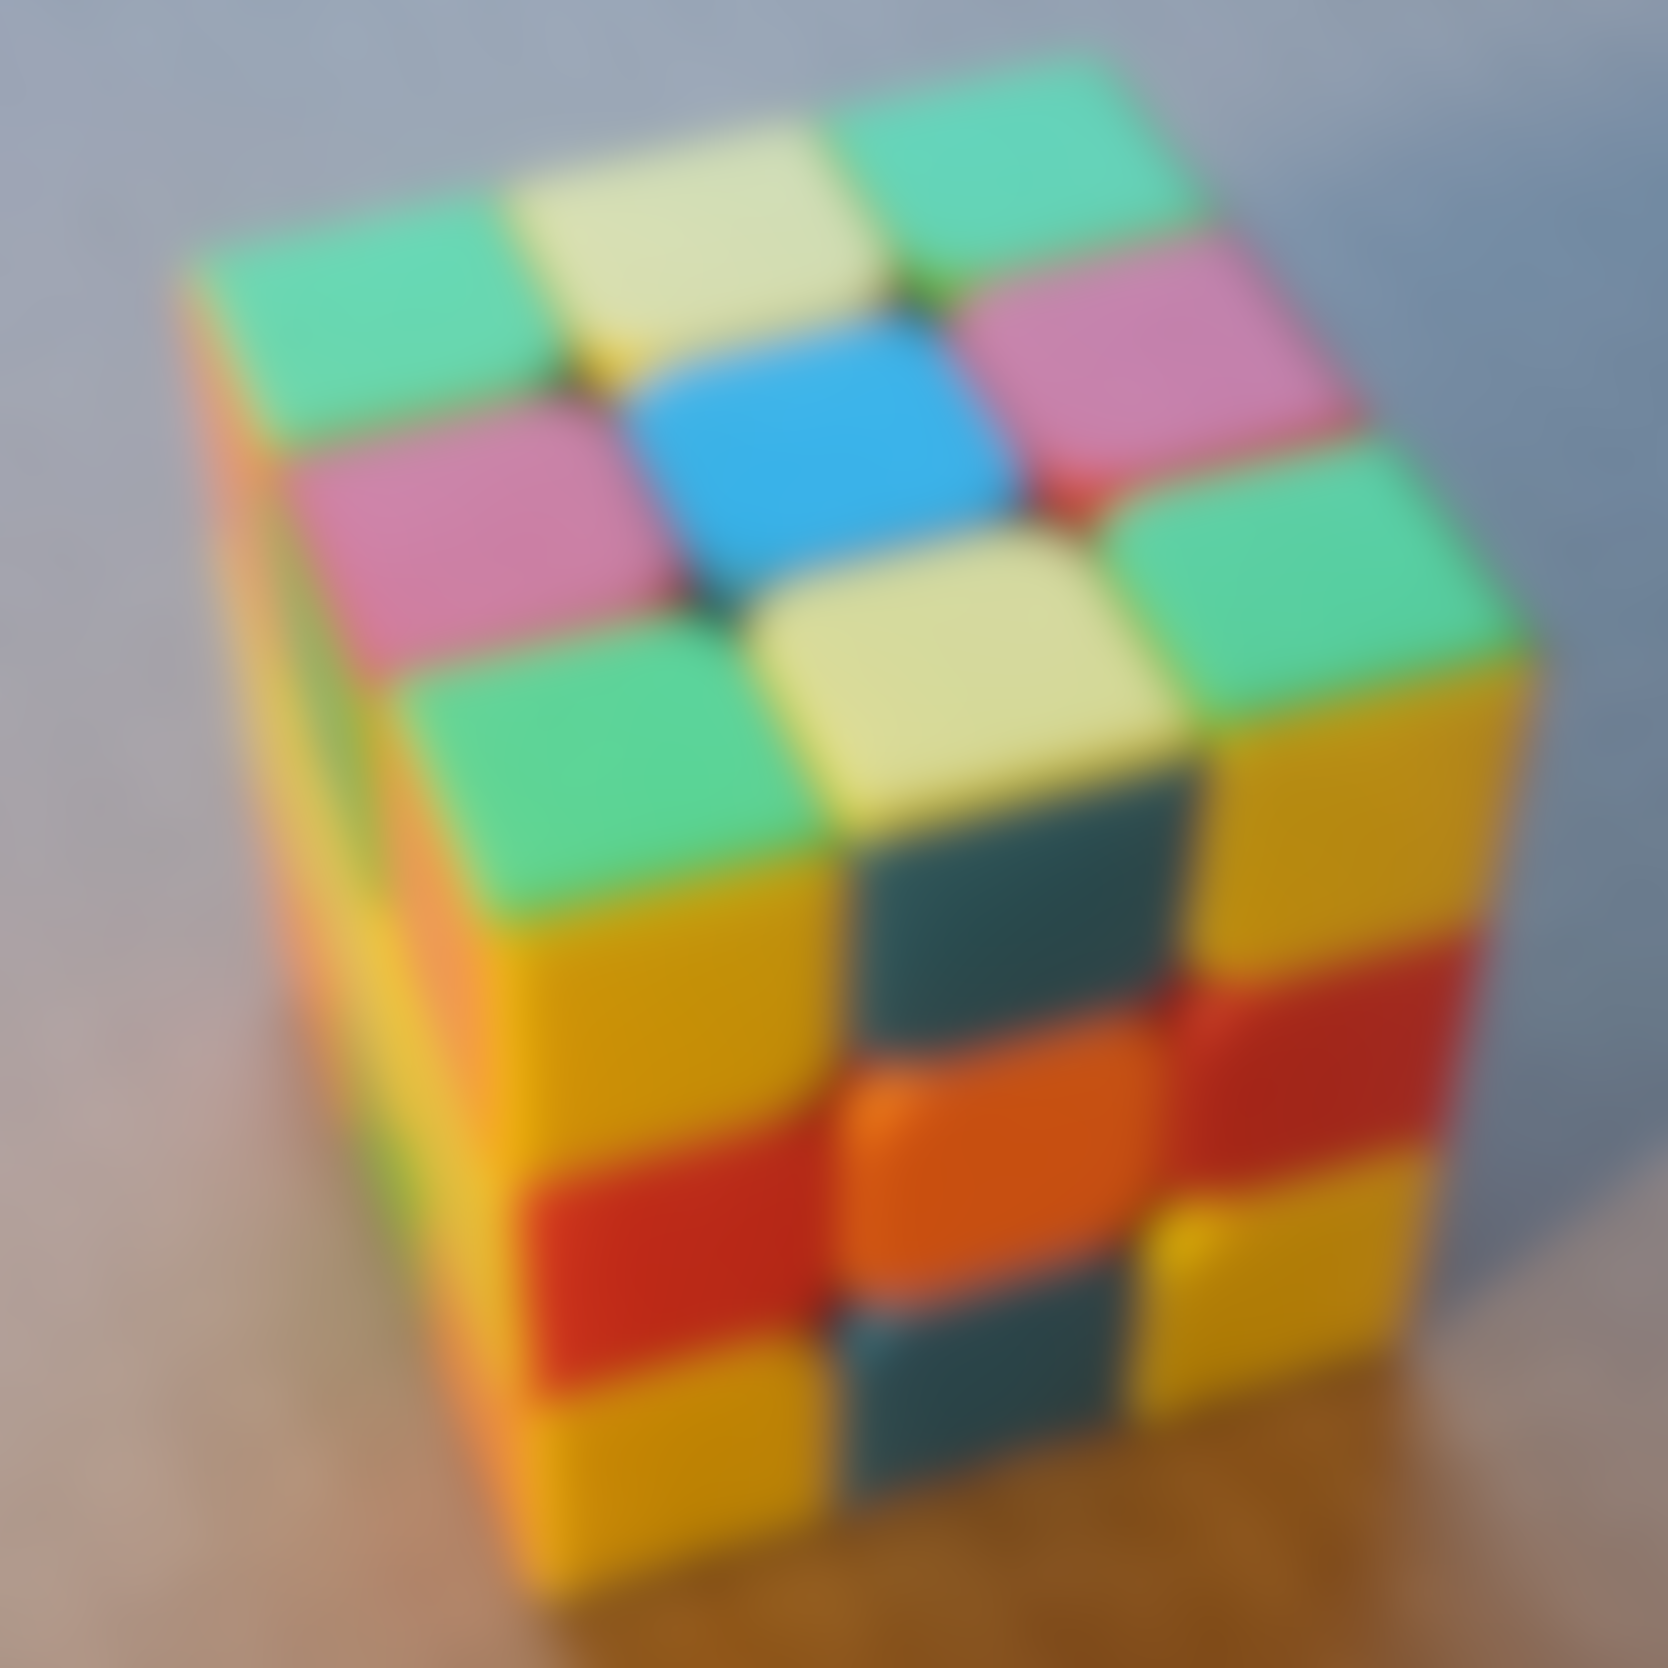
\includegraphics[width=5cm]{Gauss_blur.png}
      \caption{Obraz przed i po rozmyciu Gaussa}
      \label {fig:gauss_blur}
   \end{figure}

   Utworzenie przestrzeni skal w algorytmie \textbf{SIFT} polega na stworzemiu rodziny skal $v$ poprzez kilkukreotne skalowenie obrazu wejściowego, a następnie kilkukrotnej filtracji każdej skali $\delta$ z róźnym parametrem rozmycia $\sigma$,
   Standardowo krok skalowania wynosi $ S = 2 \: (M_{n+1} = M_{n} / 2)$, liczba skal wynosi $ n_{\delta} = 3$, a liczba poziomów rozmycia $ n_{\sigma} = 4$

\subsection{Róźnica filtrów Gaussa}:
   Funkcja \textbf{DoG} (Difference of Gaussians - Róźnica filtrów Gaussa) wyznacza obszary na obrazie które mogą zawierać elementy kluczowe (krok 2 transformacji \textbf{SIFT}). Funkcja \textbf{DoG} jest przybliżeniem \textbf{LoG} (Laplasjan filtru Gaussa) - funkcją filtrują która definiuje macierz konwolucji dla filtracji obrazu. Filtracja obrazu (Rysunek \ref{fig:DoG})  wykrywa krewędzie nie zależnie od ich skali i obrotu, w taki sposób można odrzucić obszary obrazu, dalsza analiza których jest zbędna.
   \begin{equation} \label{eq:DoG}
      \mathbf{DoG} = L(x, y, k_i \sigma) - L(x, y, k_i \sigma)
   \end{equation}
   gdzie
   \begin{equation} \label{eq:DoG}
      L(x, y, k_i \sigma) = G(x, y, k\sigma) * I(x, y)
   \end{equation}

   \begin{figure}[h]
      \centering
      \subfloat[Oryginał]{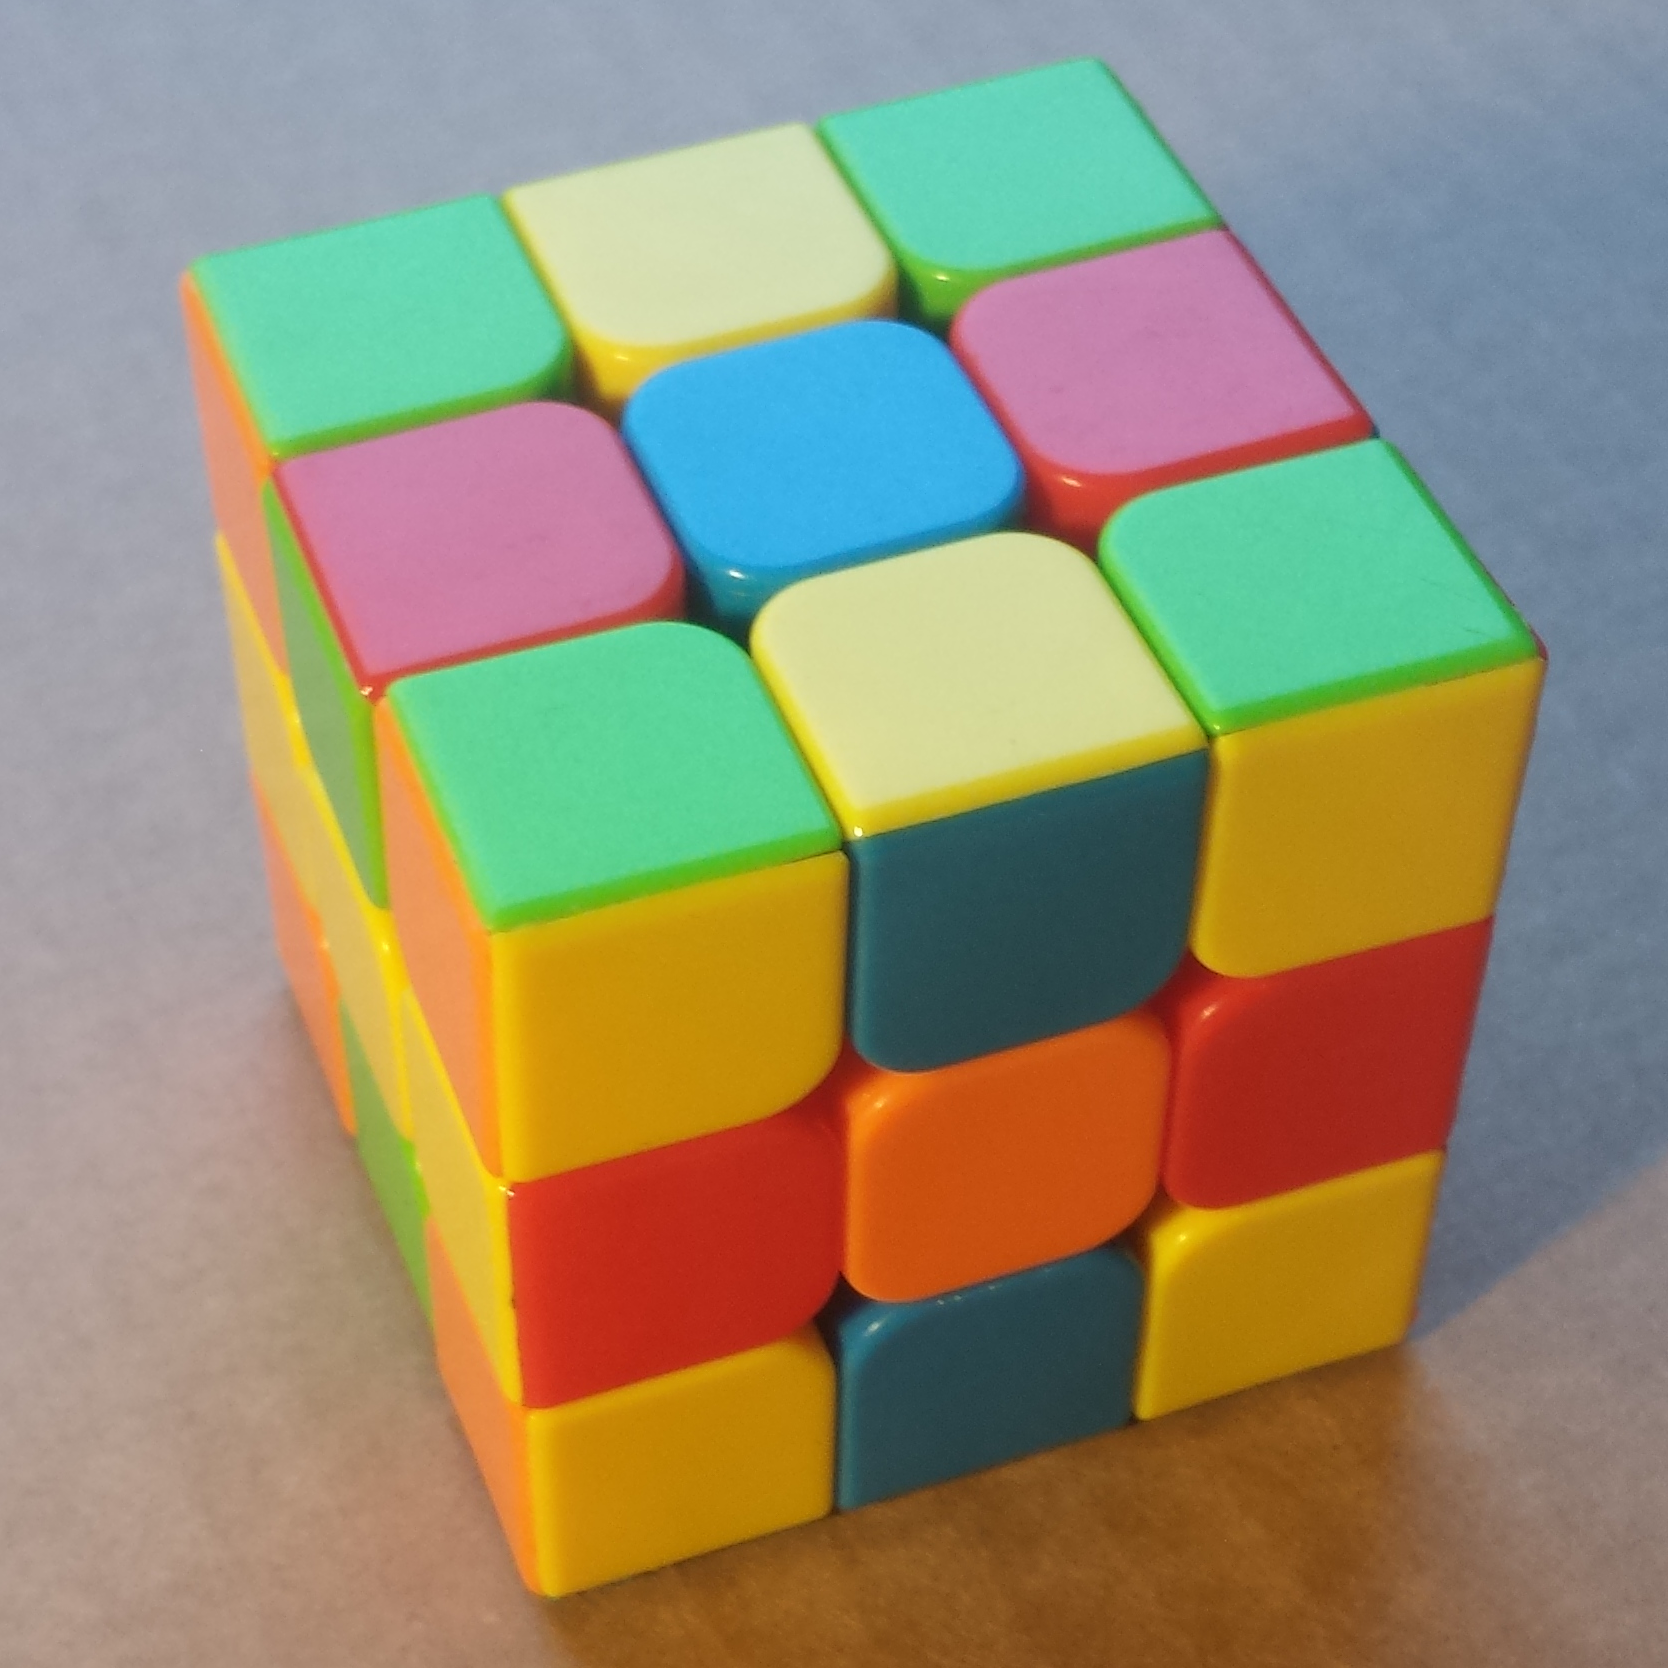
\includegraphics[width=5cm]{origin.png}}
      \smallskip{ }
      \subfloat[$\sigma_1 = 1, \sigma_2 = 4$]{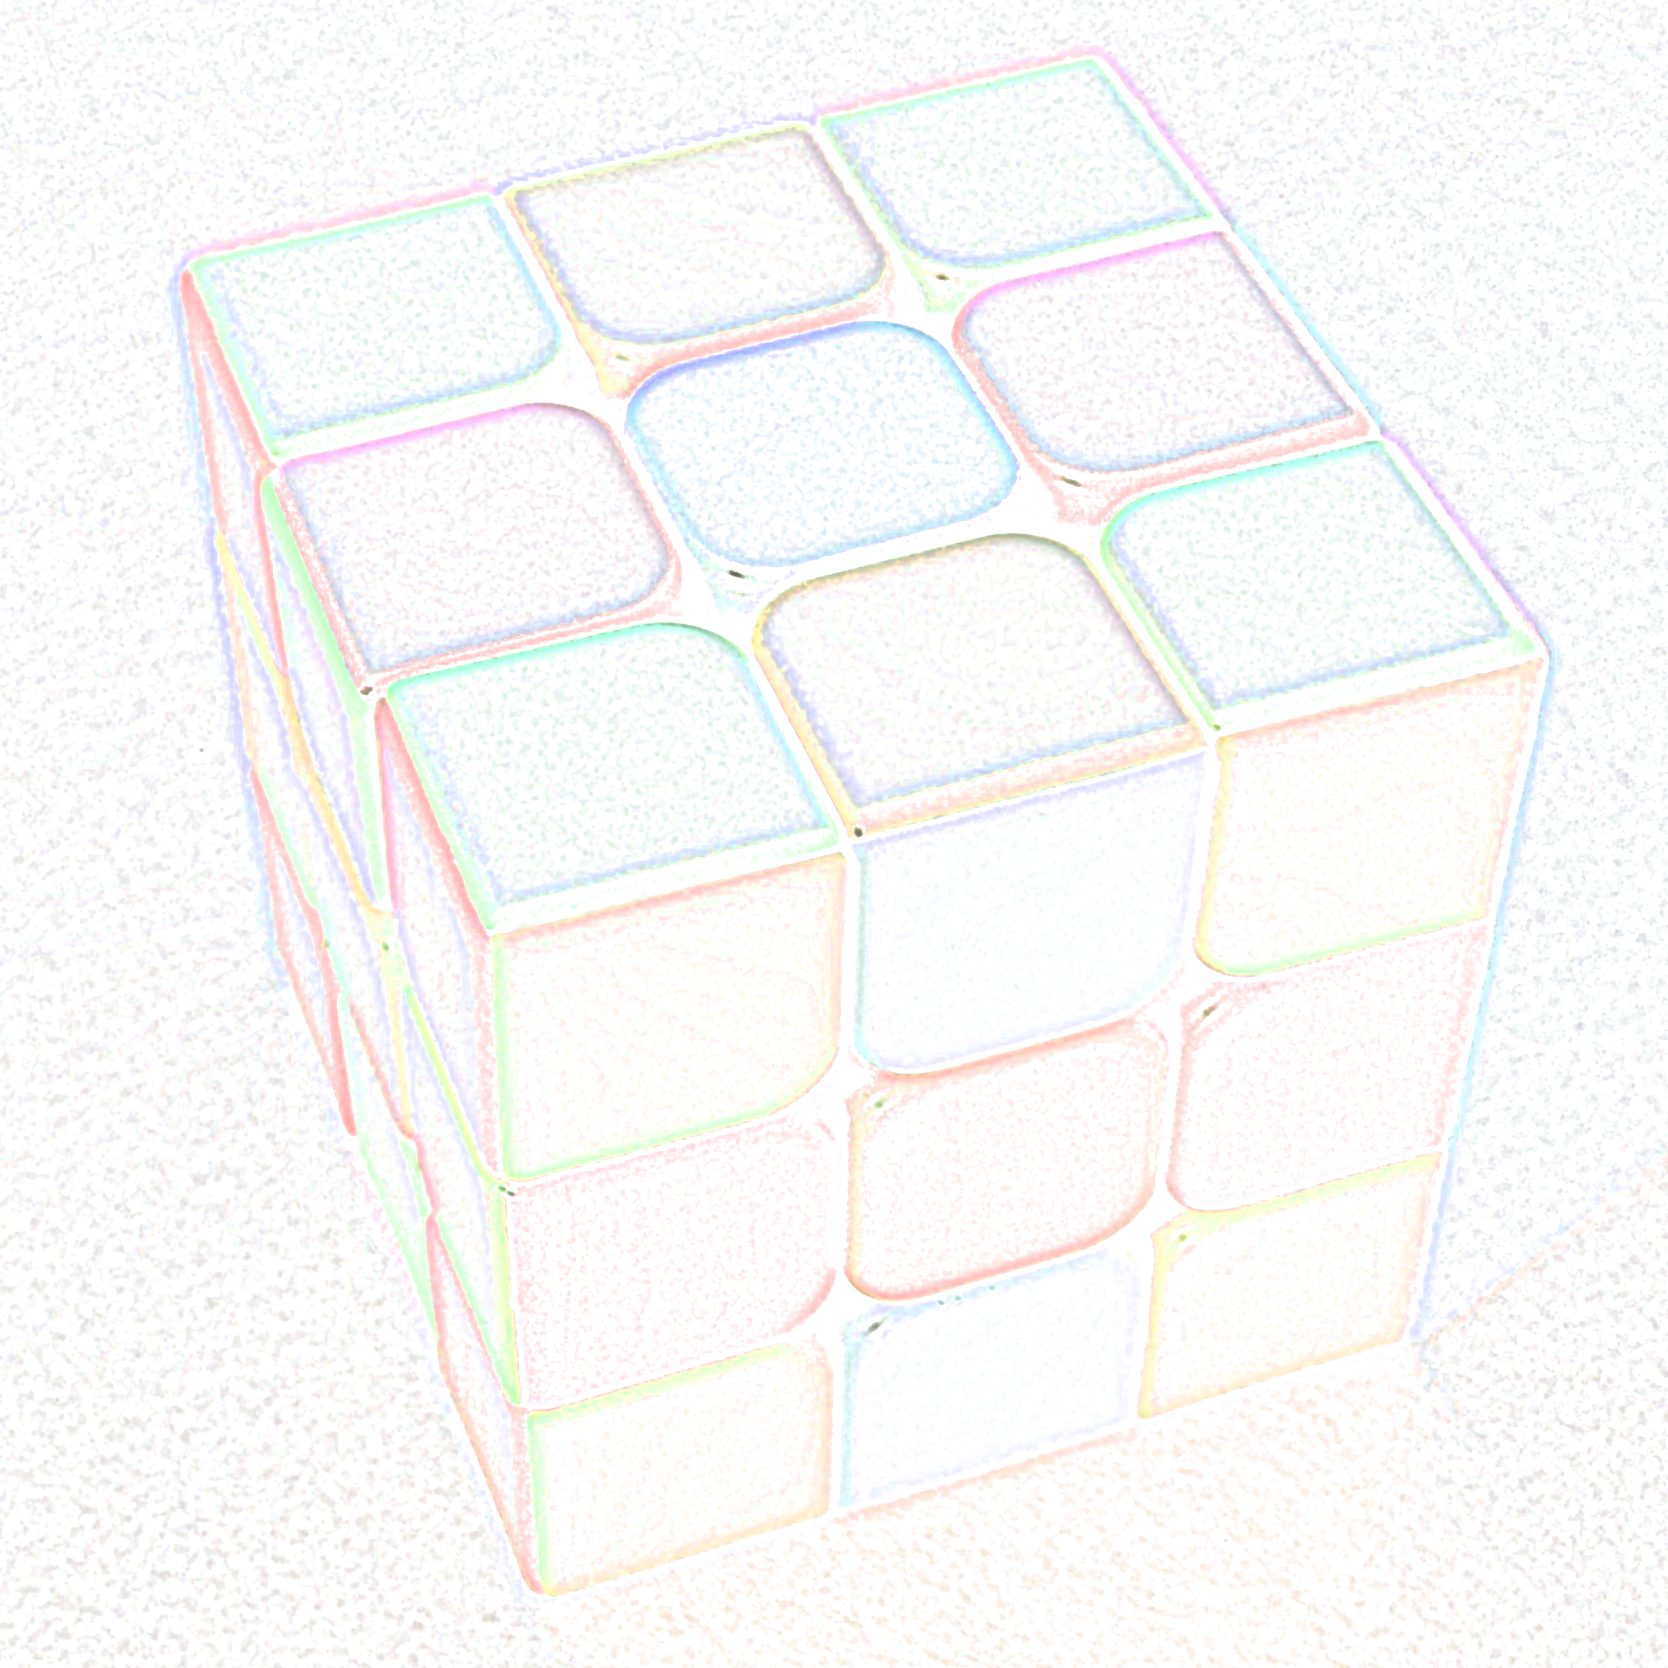
\includegraphics[width=5cm]{DoG_1to4_white.png}}
      \smallskip{ }
      \subfloat[$\sigma_1 = 2, \sigma_2 = 16$]{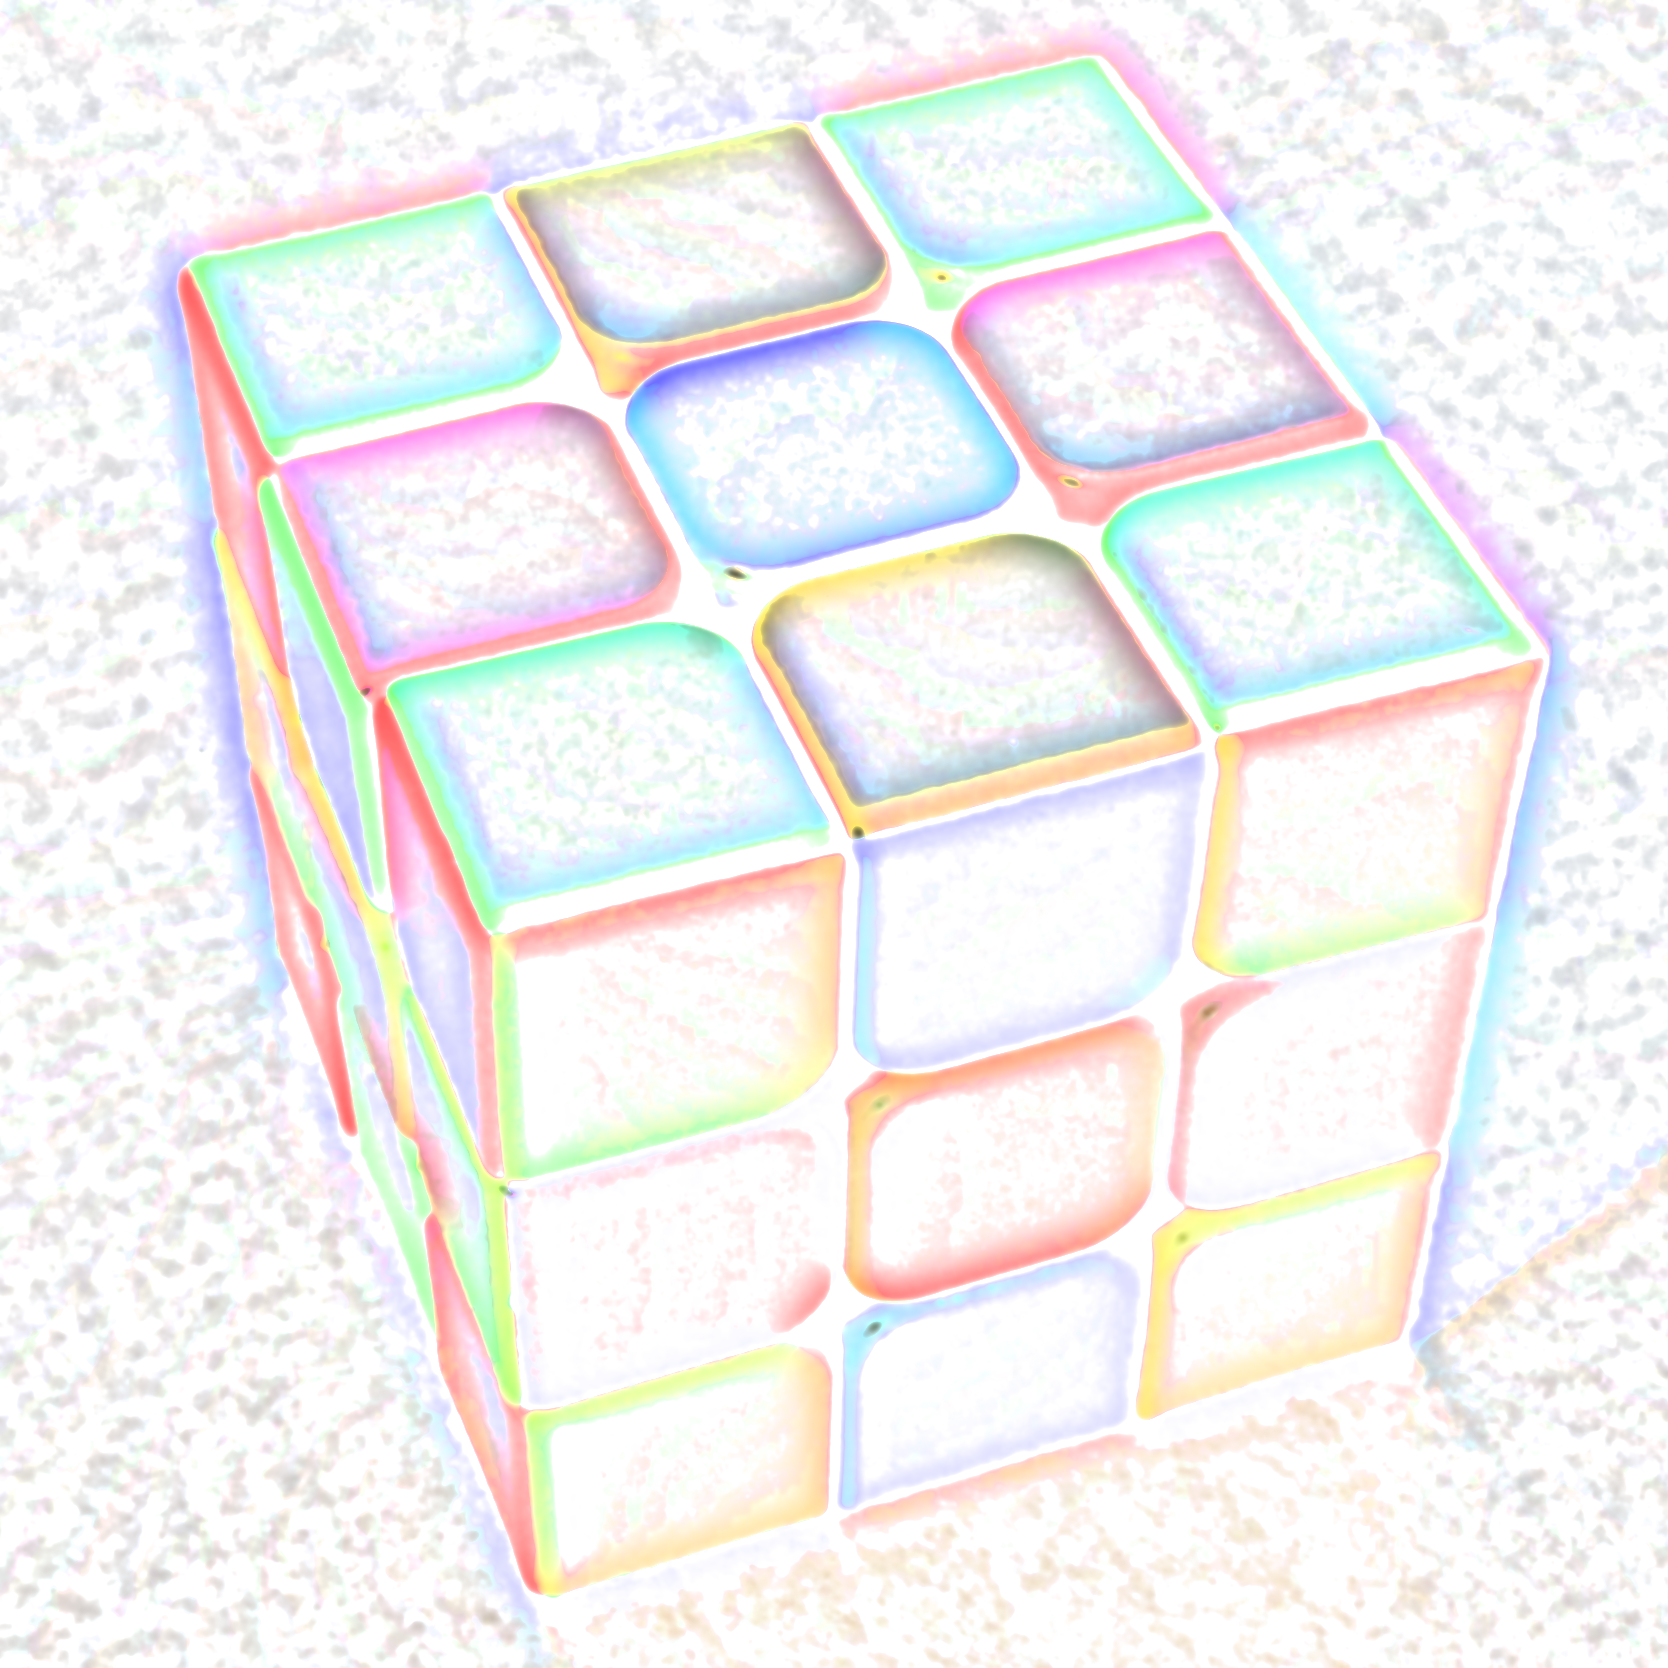
\includegraphics[width=5cm]{DoG_2to16_white.png}}
   \caption{Obraz przed i po filtracji DoG}
   \label {fig:DoG}
   \end{figure}



\subsection{Lokalizacja punktów kluczowych}
      Próba zastosowania modelu do wykrycia cechy w możliwych miejscach występowania cechy. Pozwala wykryć lokalizację i skalę elementu charakterystycznego. Wybór punktów kluczowych jest robiony na podstawie ich stabilności.

      \begin{figure}[h]
         \centering
         \includegraphics[width=5cm]{SIFT_cube_points.png}
         \label {fig:SIFT_points}
      \end{figure}

\subsection{Przydział obrotu}
      Dla każdego punktu kluczowego jest przydzielana jedna lub więcej orientacji.
      Przekształcenie elementu charakterystycznego w stosunku do lokalizacji, skali i orientacji pozwala zapewnić niezmienność transformacji cechy dla następnych operacji.
\subsection{Deskryptor punktu kluczowego}
      Transformata gradientów lokalnych

Cechy zdjęcia wykryte transformacją  \textbf{SIFT} są bardzo charakterystyczne, co pozwala z wysokim prawdopodobieństwem wykryć właściwy punkt w bazie danych innego zdjęcia.

\section{Parowanie obrazów}
Ten krok ma 2 cele:
Aby zredukować ilość błędnych par punktów charakterystycznych, kiedy 2 obrazy nie posiadają wspólnych części sceny.
Aby przyspieszyć wykonanie następnego kroku - \textbf{zestawienie punktów kluczowych}.
\section{Zestawienie punktów kluczowych}
\section{Wyznaczanie kształtów sceny}
\section{Lokalizacja kamery}




SK:
Fotogrametria

Punkt charakterystyczny
Element kluczowy
Cechy charakterystyczne
SIFT (Scale Invariant Feature Transform - Transformata )
Deskryptor

\chapter{Budowa śródowiska}

Dla praktycznego sprawdzenia zostało napisane sródowisko składające się z narzędzi:

\section{Platforma AliceVision}

\textbf{AliceVision} --- framework fotogrametryczny stworzony był aby umożliwić odtworzenie \textbf{sceny fotogrametrycznej} na podstawie zbioru zdjęć lub sekwencji klatek wideo zawierających scene.

Wybrane możliwości platformy umożliwiają:
\begin{itemize}
\item Wyznaczanie punktów charakterystycznych --- cech sceny
\item Parowanie zdjęć --- para jest tworzony gdy zdjęcia zawierają ten sam obiekt
\item Zestawienie cech zdjęć
\item Odtworzenie struktury cech w przestrzeni 3D
\item Lokalizacja względna i bezwzględna kamery
\item Kalibracja kamery
\item Utworzenie mapy głębokości sceny
\item Odworzenie powierzchni obiektów sceny
\item Teksturowanie obiektów sceny
\end{itemize}

\subsection{CameraInit}
\subsection{FeatureExtraction}
Najwiej
\subsection{ImageMatching}
\subsection{FeatureMatching}
\subsection{StructureFromMotion}
\section{Implementacja śródowiska}
\begin{itemize}
\item przetwarzania danych wejściowych w celu zestawienia zdjęć i lokalizacji kamery
\item wyświetlania wyników fotogrametrycznych i położenia kamery w przestrzeni
\item wyświetlania elementów kluczowych w przestrzeni i odpowiednich obrazach
\item przeprowadzania testów wydajności dla róźnych zestawów danych i parametrów przetwarzania
\end{itemize}

\subsection{Pipeline}
\subsection{Rysowanie}
\subsection{Pomiar czasu}

\graphicspath{ {./img/data/} }

\chapter{Przebieg badań}

W badaniu przeprowadzona analiza wyników przetwarzania zestawów zdjęć, każdy zestaw przedstawia następujące sceny:
\begin{itemize}
   \item Kostka Rubika na podstawce, "c0" (Rysunek \ref{fig:scene_c0}).
   \item Kostka Rubika z oświetleniem zmiennym, "c1" (Rysunek \ref{fig:scene_c1}).
   \item Kostka Rubika z oświetleniem punktowym, "c2" (Rysunek \ref{fig:scene_c2}).
   \item Znaki specjalne, "mark" (Rysunek \ref{fig:scene_mark}).
   \item Budynek A1 PWr (wybrzeże Wyspiańskiego 27), "A1" (Rysunek \ref{fig:scene_A1}).
\end{itemize}

\begin{figure}[h]
   \centering
   \includegraphics[width=6cm]{img/c0.jpg}
   \caption{Kostka Rubika na podstawce, scena "c0", 4 zdjęcia}
   \label {fig:scene_c0}
\end{figure}
\begin{figure}[h]
   \centering
   \includegraphics[width=6cm]{img/c1.jpg}
   \caption{Kostka Rubika z oświetleniem zmiennym, scena "c1", 20 zdjęć}
   \label {fig:scene_c1}
\end{figure}
\begin{figure}[h]
   \centering
   \includegraphics[width=6cm]{img/c2.jpg}
   \caption{Kostka Rubika z oświetleniem punktowym, scena "c2", 10 zdjęć}
   \label {fig:scene_c2}
\end{figure}
\begin{figure}[h]
   \centering
   \includegraphics[width=6cm]{img/mark.jpg}
   \caption{Znaki specjalne, scena "mark", 13 zdjęć}
   \label {fig:scene_mark}
\end{figure}
\begin{figure}[h]
   \centering
   \includegraphics[width=6cm]{img/A1.jpg}
   \caption{Budynek A1 PWr, scena "A1", 19 zdjęć}
   \label {fig:scene_A1}
\end{figure}

Wyniki są wygenerowane w następujących postaciach:
\begin{itemize}
   \item Rekonstrukcja sceny w przestrzenie trójwymiarowej, zawiera zbiór punktów kluczowych i wykrytych pozycji kamery wraz. Nazwa pozycji odpowiada nazwie pliku zdjęcia.
   \item Oznaczone wspólne punkty kluczowe dla wybranych zdjęć. Na rekonstrukcji sceny punkty są oznaczone gwiazdką i promieniem cągnącym się promieniem od miejsca kamery wraz z przydzieloną literą. Na zdjęciu punkty są oznaczone fioletowym fioletowym kółkiem i odpowiednią literą.
   \item Wykres zależności czasu wykonywania, procentu wykrytych ujęć i powodzenia na etapie rekonstrukcji sceny od ustawień parametru transformacji SIFT.
   \begin{itemize}
      \item  Na czerwono: czas w sekundach
      \item  Na niebiesko: wykryte ujęcia w procentach
      \item  Na zielono: procent udanych prób rekonstrukcji sceny, może przyjmować wartość 0 (próba nieudana) lub 100 (rekonstrukcja powiodła się), wartość pomiędzy 0 a 100 oznaczała by błąd pod czas wykonywania pomiarów.
   \end{itemize}
\end{itemize}

\section{Odtwarzanie sceny z róźną zawartością. Wykrycie i dopasowanie cech}
\begin{figure}[h]
   \centering
   \includegraphics[width=5cm]{feature_mark/03.png}
   \includegraphics[width=5cm]{feature_mark/07.png}
   \caption{Wybrane punkty charakterystyczne, zdjęcie 03 i 07, scena "mark"}
   \label {fig:feature_mark_03_07}
\end{figure}

\begin{figure}[h]
   \centering
   \includegraphics[width=10cm]{feature_mark/scene.png}
   \caption{Wybrane punkty charakterystyczne, scena "mark"}
   \label {fig:feature_mark_plot}
\end{figure}

\begin{figure}[h]
   \centering
   \includegraphics[width=10cm]{feature_A1/plot.png}
   \caption{Wybrane punkty charakterystyczne, scena "A1"}
   \label {fig:feature_A1_plot}
\end{figure}

\begin{figure}[h]
   \centering
   \includegraphics[width=10cm]{feature_A1/img_0.png}
   \caption{Wybrane punkty charakterystyczne, zdjęcie 0, scena "A1"}
   \label {fig:feature_A1_img_0}
\end{figure}
\begin{figure}[h]
   \centering
   \includegraphics[width=10cm]{feature_A1/img_10.png}
   \caption{Wybrane punkty charakterystyczne, zdjęcie 10, scena "A1"}
   \label {fig:feature_A1_img_10}
\end{figure}
\begin{figure}[h]
   \centering
   \includegraphics[width=10cm]{feature_A1/img_15.png}
   \caption{Wybrane punkty charakterystyczne, zdjęcie 15, scena "A1"}
   \label {fig:feature_A1_img_15}
\end{figure}

   Dla dwóch zestawów "A1" i "mark" przeprowadzono odtwarzanie sceny przy takich samych parametrach używając scryptu .

   Scena "mark" przedstawia sobą cztery czarne znaki charakterystyczne na białym tle.
   Scena była specjalnie sprojektowana, aby sprawdzić zachowanie algorytmu \textbf{SIFT}.

   Punkty charakterystyczne na rysunku \ref{fig:feature_mark_03_07} są umieszczone na wierzchołkach znaku, co zgadza się z algorytmem, gdyż w tych miejscach występują ekstrema funkcji \textbf{DoG}.
   Brak punktów na krawędziach spowodowany jest jednym z kroków filtracji \textbf{SIFT} punktów na krawędziach.

   Charakterystyczną róźnicą odtwarzanych scen "A1" (Rysunek \ref{fig:feature_A1_plot}) i "mark" (Rysunek \ref{fig:feature_mark_plot}) pod względem wykrytych punktów kluczowych jest znacznie mniejszą ilość odnalezionych cech dla sceny "mark".
   Taka róźnica jest skutkiem ograniczonej ilości elementów które mogły by spełnić kryteria transformaty \textbf{SIFT}.

   Dodatkowo można odznaczyć bardzo dobry wynik jak zestawienia punktów kluczowych dla sceny "A1" (Rysunek \ref{fig:feature_A1_img_0} - \ref{fig:feature_A1_img_15}) przy tak dużej liczbie elementów kluczowych, jak i dokładność wyznaczonych kształtów sceny (Rysunek \ref{fig:feature_mark_plot}, \ref{fig:preset_mark_normal} - \ref{fig:preset_mark_ultra}) --- zdjęcia sceny "mark" rzeczywiście były robione przemieszczaniem kamery wzdłuż prostej.

\section{Wpływ parametrów rozpoznawania cech na wynik}
\begin{figure}[h]
   \centering
   \includegraphics[width=10cm]{preset_c2/normal.png}
   \caption{Odtwarzana scena "c2", parametr: normal}
   \label {fig:preset_c2_normal}
\end{figure}
\begin{figure}[h]
   \centering
   \includegraphics[width=10cm]{preset_c2/high.png}
   \caption{Odtwarzana scena "c2", parametr: high}
   \label {fig:preset_c2_high}
\end{figure}
\begin{figure}[h]
   \centering
   \includegraphics[width=10cm]{preset_c2/ultra.png}
   \caption{Odtwarzana scena "c2", parametr: ultra}
   \label {fig:preset_c2_ultra}
\end{figure}

\begin{figure}[h]
   \centering
   \includegraphics[width=10cm]{preset_mark/normal.png}
   \caption{Odtwarzana scena "mark", parametr: normal}
   \label {fig:preset_mark_normal}
\end{figure}
\begin{figure}[h]
   \centering
   \includegraphics[width=10cm]{preset_mark/high.png}
   \caption{Odtwarzana scena "mark", parametr: high}
   \label {fig:preset_mark_high}
\end{figure}
\begin{figure}[h]
   \centering
   \includegraphics[width=10cm]{preset_mark/ultra.png}
   \caption{Odtwarzana scena "mark", parametr: ultra}
   \label {fig:preset_mark_ultra}
\end{figure}

\begin{figure}[h]
   \centering
   \includegraphics[width=10cm]{preset_A1/medium.png}
   \caption{Odtwarzana scena "A1", parametr: medium}
   \label {fig:preset_A1_medium}
\end{figure}
\begin{figure}[h]
   \centering
   \includegraphics[width=10cm]{preset_A1/normal.png}
   \caption{Odtwarzana scena "A1", parametr: normal}
   \label {fig:preset_A1_normal}
\end{figure}
\begin{figure}[h]
   \centering
   \includegraphics[width=10cm]{preset_A1/high.png}
   \caption{Odtwarzana scena "A1", parametr: high}
   \label {fig:preset_A1_high}
\end{figure}
\begin{figure}[h]
   \centering
   \includegraphics[width=10cm]{preset_A1/ultra.png}
   \caption{Odtwarzana scena "A1", parametr: ultra}
   \label {fig:preset_A1_ultra}
\end{figure}

Pierwszy krok procesu fotogrametrycznego - rozpoznawanie cech można dokonać z róźnym parametrem ustawień transformaty SIFT.
Taki parametr, nazywany "preset" może przyjąć jedną z wartości ["low", "medium", "normal", "high", "ultra"].
Rysunki \ref{fig:measure_c0} - \ref{fig:measure_A1} posiadają wyniki wykonywań procesu fotogrametrycznego dla róźnych ustawień.
Dla przeciętnej sceny stosowanie ustawień "low" i "medium" zwykle było niewystarczające aby wykryć jakiekolwiek pozycje kamery.
Ustawienie "normal" okazało się wystarczającym aby wykryć 80\% pozycji. Ustawienia "high" i "ultra" pozwalają uzyskać najlepszy wynik, jednak stosowanie takich ustawień skutkuje znacznym wydłużeniem czasu obliczenia.

Dogłębne wyszukiwanie cech może wykryć więcej punktów kluczowych w scenach z wysoką entropią, np. dla sceny "A1", "c2", rekonstruowane sceny 3D (Rysunek \ref{fig:preset_c2_normal} - \ref{fig:preset_c2_ultra}, \ref{fig:preset_A1_medium} -  \ref{fig:preset_A1_ultra}) których posiadają charakterystyczny wzrost wykrytych cech wraz z wzrostem parametrem "preset".


Swoją drogą dla sceny "mark" --- sceny o niskiej entropii zbiór cech pozostaje praktycznie niezmienny (Rysunek \ref{fig:preset_mark_normal} - \ref{fig:preset_mark_ultra})


Skutkiem ubocznym stosowania wyższych ustawień można uważać zwiększenie szumu (błędnie wykrytych i źle zlokalizowanych cech wspólnych) w scenach z duża ilością obiektów (Rysunek \ref{fig:preset_A1_normal}, \ref{fig:preset_A1_high}, \ref{fig:preset_A1_ultra}).

Zestaw "c1" posiada zdięcia przy róźnym oświetleniu --- część zdjęć była zrobiona z dodatkowym źródłem światła.
Można zauważyć, że rekonstrukcja sceny powiodła się dopiero przy większej liczbie cech, przy większym ustawieniu "high" (w porównaniu do innych zestawów odtwarzanie sceny następowało przy mniejszym nastawieniu), przy czym nawet przy ustawieniu "ultra", część pozycji wciąż nie jest odtwarzona.
Jednym z warunków dobrego wyniku fotogrametrycznego jest niezmienność sceny w trakcie robienia zdjęć, w tym oświetlenia.

\section{Czas obliczenia}

Rysunki \ref{fig:measure_c0} - \ref{fig:measure_A1} przedstawiają zależności czasu od ustawień transformaty \textbf{SIFT}.
Zmiana parametrów transformaty wykrywającej cechy ma bezpośredni wpływ na czas potrzebny do wykrycia cech i pośredni dla parowania cech i odtwarzania sceny, gdyż dokładniejsze wyszukiwanie cech zwiększa liczbę znalezionych punktów kluczowych.
Wyjątek stanowią sceny z ograniczoną liczbą elementów.
Na przykład dla sceny "mark" liczba wykrytych elementów przy ustawieniach "normal" i "high" nie zmienia się. Wzrost czasu przy ustawieniu "ultra" jest powiązany wzrostem szumu (błędnie wykrytych punktów charakterystycznych).

Bezpośredni wpływ na czas obliczenia również stanowi licza zdjęć.
Czas potrzebny na przetworzenie zestawu zdjęć wzrasta wraz z liczbą ujęć.

\begin{figure}[h]
   \centering
   \includegraphics[width=7cm]{measure/c0.png}
   \caption{Czas wykonania, scena "c0"}
   \label {fig:measure_c0}
\end{figure}
\begin{figure}[h]
   \centering
   \includegraphics[width=7cm]{measure/c1.png}
   \caption{Czas wykonania, scena "c1"}
   \label {fig:measure_c1}
\end{figure}
\begin{figure}[h]
   \centering
   \includegraphics[width=7cm]{measure/c2.png}
   \caption{Czas wykonania, scena "c2"}
   \label {fig:measure_c2}
\end{figure}
\begin{figure}[h]
   \centering
   \includegraphics[width=7cm]{measure/mark.png}
   \caption{Czas wykonania, scena "mark"}
   \label {fig:measure_mark}
\end{figure}
\begin{figure}[h]
   \centering
   \includegraphics[width=7cm]{measure/A1.png}
   \caption{Czas wykonania, scena "A1"}
   \label {fig:measure_A1}
\end{figure}

\chapter{Podsumowanie}

W trakcie wykonywania pracy inżynierskiej udało się zbudować zestaw narzędzi (śródowisko), które umożliwia uruchomienie procesu lokalizacji fotogrametrycznej, wyświetlenie wyników lokalizacji, odtwarzanie sceny w przestrzeni trójwymiarowej. Dodatkowo śródowisko posiada narzędzie dla przeprowadzania testów wydajności dla róźnych zestawów danych i róźnych parametrów przetwarzania.

Przedstawione śródowisko wykorzystuje platformę AliceVision dla implementacji procesu fotogrametrycznego.
Platforma ta została wybrana dla potrzeb projektu, ponieważ jest dobrze opracowanym i potężnym frameworkiem z ciągle podtrzymywanym i otwartym kodem źródłowym.
Do wad frameworku można odnieść częściowy brak dokumentacji i dość skomplikowany proces kompilacji frameworku w śródowisku własnym.

Dla praktycznego sprawdzenia zaproponowanej teorii lokalizacji zostały dobrane pięć zestawów zdjęć zawierające róźne sceny.
Sceny czterech z pięciu zestawów zawierały zestaw obiektów (kostka Rubika, arkusz zawierający znaki specjalne), jedna scena zawierała otoczenie (duży budynek).


Można powiedzieć, że proces przetwarzania zdjęć jest dość wymagający pod względem zapotrzebowania zasobów obliczeniowych.
Obliczenia były przeprowadzane na przeciętnym sprzęcie obliczeniowym dla roku 2020 --- procesor Intel i7-2620m.

Dla zestawu o rozmiarze 10 zdjęć potrzebne jest około 40 sekund na uzyskanie zadowalającego wyniku.
Dla zestawu o rozmiarze 4 zdjęć uzyskanie zadowalającego wyniku zajeło 4 sekundy.

Ponieważ czas obliczenia wzrasta wraz ze wzrostem nastawienień parametrów przetwarzania i wraz ze wzrostem ilości danych, dla dużych zestawów danych proponowana jest próba stosowania niższych parametrów na początek, a następnie stopniowe zwiększenie ustawień aż do momentu uzyskania zadowalających wyników. Dodatkowo można wprowadzić filtrację wstępną obrazów złej jakości i zbędnej zawartości.

Uzyskanie dobrego wyniku lokalizacji (stosunek wykrytych pozycji do liczby zdjęć) wprost zależy od liczby cech charakterystycznych na zdjęciach.
Przykładem dobrego wyniku można uważać przetwarzanie zestawu "A1", zdjęcia którego mają wysoki poziom entropii.


Dla 4 z 5 zestawów proces lokalizacji zakończył się powodzeniem, pozostały zestaw posiadał zdjęcia przy róźnym oświetleniu i część ujęć nie została wykryta. Aby uzyskać najlepszy wynik scena fotogrametryczna powinna być niezmienna w trakcie robienia zdjęć.

Zastosowany algorytm pozwala na względną lokalizację, oznacza to, że rzeczywiste położenie i odległości pozostają nieznane. Aby móc na podstawie opisanego algorytmu uzyskać lokalizację absolutną należy wprowadzić skalę (na przykład przez zmierzenie jednego z obiektów sceny) i wprowadzić układ odniesienia do sceny.

\addcontentsline{toc}{chapter}{\bibname}

\begin{thebibliography}{9}
\bibitem{latexcompanion}
Michel Goossens, Frank Mittelbach, and Alexander Samarin.
\textit{The \LaTeX\ Companion}.
Addison-Wesley, Reading, Massachusetts, 1993.

\bibitem{einstein}
Albert Einstein.
\textit{Zur Elektrodynamik bewegter K{\"o}rper} . (German)
[\textit{On the electrodynamics of moving bodies}].
Annalen der Physik, 322(10):891–921, 1905.

\bibitem{knuthwebsite}
Knuth: Computers and Typesetting,
\\\texttt{http://www-cs-faculty.stanford.edu/\~{}uno/abcde.html}
\end{thebibliography}

AV:
https://github.com/alicevision/AliceVision
%https://alicevision.org/#photogrammetry
https://github.com/alicevision/meshroom-manual

SIFT:
[Distinctive Image Featuresfrom Scale-Invariant Keypoints]
https://www.cs.ubc.ca/~lowe/papers/ijcv04.pdf

[Anatomy of the SIFT Method]
http://www.ipol.im/pub/art/2014/82/

[OpenCV]
%https://opencv-python-tutroals.readthedocs.io/en/latest/py_tutorials/py_feature2d/py_sift_intro/py_sift_intro.html

Python 3.7:
https://matplotlib.org/
https://docs.python.org/3/library/argparse.html
https://docs.python.org/3/library/json.html

SfM:
P. Moulon, P. Monasse and R. Marlet. Adaptive Structure from Motion with a contrario model estimation. ACCV 2012.

M. Jancosek, T. Pajdla. Multi-view reconstruction preserving weakly-supported surfaces. CVPR 2011.



?:
SIFT:
https://aishack.in/tutorials/sift-scale-invariant-feature-transform-introduction/
https://medium.com/analytics-vidhya/introduction-to-sift-scale-invariant-feature-transform-65d7f3a72d40

%https://en.wikipedia.org/wiki/Scale-invariant_feature_transform
%https://commons.wikimedia.org/wiki/File:Sift_keypoints_filtering.jpg?uselang=ru
DoG:
http://aragorn.pb.bialystok.pl/~boldak/DIP/CPO-W04-v01-50pr.pdf


%\appendix
%\chapter{Dodatek}


\end{document}
